\documentclass[12pt, a4paper]{report}
\usepackage[utf8]{inputenc}
\newcommand\preamble{
    \usepackage[italian]{babel}
    \usepackage{geometry}
    \usepackage{amsmath}
    \usepackage{amssymb}
    \usepackage{graphicx}
    \usepackage{ulem}
    \geometry{margin=2cm}
    \usepackage{listings}
    \let\olditemize\itemize
    \renewcommand\itemize{\olditemize\setlength\itemsep{0em}}
}
% Definizione delle variabili
\newcommand{\imagePath}{Immagini/logoUni.png}

% Definizione del comando per la pagina di titolo con argomenti
\newcommand{\customTitlePage}[5]{
    \newcommand{\courseTitle}{#1}
    \newcommand{\authorName}{#2}
    \newcommand{\academicYear}{#3}
    \newcommand{\universityName}{#4}
    
    \begin{titlepage}
        \centering
        \includegraphics[width=0.5\textwidth]{\imagePath}\par\vspace{1cm}
        {\scshape\LARGE \universityName \par}
        \vspace{1.5cm}
        {\huge\bfseries \courseTitle \par}
        \vspace{2cm}
        {\Large\itshape \authorName \par}
        \vfill
        \academicYear
    \end{titlepage}
}

\preamble

\begin{document}
\customTitlePage{Fondamenti di Computazione Quantistica}{Lorenzo Vaccarecci}{Anno Accademico 2024/2025}{Università degli Studi di Genova}
\newpage
\tableofcontents
\chapter{Introduzione}
\section{Porte logiche universali}
\begin{itemize}
    \item \texttt{NOT(A)} $\equiv \bar{A}$
    \item \texttt{AND(A,B)} $\equiv A \cdot B$ oppure $A \land B$
    \item \texttt{OR(A,B)} $\equiv A + B$ oppure $A \lor B$
    \item \texttt{XOR(A,B)} $\equiv A \oplus B = (A+B) \mod 2$
    \item \texttt{NAND(A,B)} $\equiv \bar{A \cdot B}$ oppure $\bar{A \lor B}$
    \item \texttt{NOR(A,B)} $\equiv \bar{A + B}$ oppure $\bar{A \land B}$
\end{itemize}
L'insieme di \texttt{AND} e \texttt{NOT} oppure di \texttt{OR} e \texttt{NOT} sono insiemi universali. Questo significa che, ad esempio, usando solo combinazioni di porte \texttt{AND} e \texttt{NOT} è possibile implementare una qualsiasi funzione booleana. Pur formando set universali, le porte \texttt{AND}, \texttt{OR}, \texttt{NAND} e \texttt{NOR} sono però \textbf{irreversibili}. A livello concettuale è interessante introdurre delle porte logiche che siano \textbf{reversibili}. Questo vuol dire che se combiniamo in sequenza una porta logica reversibile con la sua inversa, riotteniamo l'informazione originale. La porta di Fredkin può essere interpretata come uno \textit{switch} controllato di bit. Il bit di controllo è \texttt{A}; se questo è acceso i bit \texttt{B} e \texttt{C} vengono scambiati, altrimenti vengono lasciati identici.
\begin{center}
    \begin{tabular}{|c|c|c|c|c|c|}
    \hline
    \texttt{A} & \texttt{B} & \texttt{C} & \texttt{Out1} & \texttt{Out2} & \texttt{Out3} \\
    \hline
    0 & 0 & 0 & 0 & 0 & 0 \\
    \hline
    0 & 0 & 1 & 0 & 0 & 1 \\
    \hline
    0 & 1 & 0 & 0 & 1 & 0 \\
    \hline
    0 & 1 & 1 & 0 & 1 & 1 \\
    \hline
    1 & 0 & 0 & 1 & 0 & 0 \\
    \hline
    1 & 0 & 1 & 1 & 1 & 0 \\
    \hline
    1 & 1 & 0 & 1 & 0 & 1 \\
    \hline
    1 & 1 & 1 & 1 & 1 & 1 \\
    \hline
    \end{tabular}
    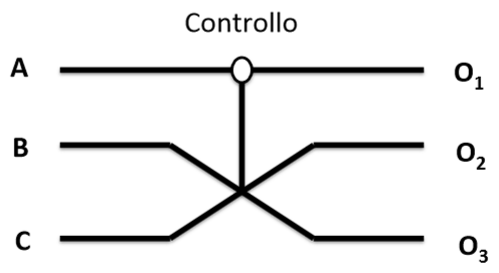
\includegraphics[width=0.4\textwidth]{Immagini/fredkin_circuit.png}
\end{center}
\section{Operazioni Bit-a-Bit}
A una stringa di $n$ bit possiamo associare un intero compreso fra 0 e $N-1$ con $N=2^n$. All'intero $x$ associamo la stringa di bit $x_0x_1x_2\dots x_{n}$ con $x_{i}=0,1 \text{ e } i=0,1,\dots,n$ tale che $x=\sum_{i=0}^{n}x_{i}2^{n-i}$. Possiamo codificare $N=2^{n}$ interi ma questi saranno compresi fra 0 e $N-1=2^{n}-1$.
\subsection{Prodotto interno bit-per-bit}
\begin{equation*}
    x\cdot z \equiv (x_{1}z_{1} + x_{2}z_{2} + \dots + x_{n}z_{n}) \mod 2
\end{equation*}
E' anche chiamato prodotto \texttt{AND} bitwise perchè si ottiene prendendo le operazioni \texttt{AND} fra i singoli bit.
\subsection{Somma bit-per-bit: bitwise \texttt{XOR}}
Indichiamo con $x\oplus z$ la somma bit-per bit, modulo 2. Il risultato questa volta è una stringa il cui $i$-esimo bit ha il valore $x_{i}+z_{i} \mod 2 = x_{i} \text{ \texttt{XOR} } z_{i}$.
\section{Prerequisiti matematici}
\subsection{Numeri complessi}
Ogni numero complesso $z\in \mathbb{C}$ può essere scritto come $z=a+ib$, con $a\in \mathbb{R}$ \textbf{parte reale} e $b\in \mathbb{R}$ \textbf{parte immaginaria}. Se $z=a+ib$ e $w=c+id$, abbiamo
\begin{equation*}
    z+w = (a+c) + i(b+d)
\end{equation*}
\begin{equation*}
    z\cdot w = (ac-bd) + i(ad+bc)
\end{equation*}
Per ogni $z\in \mathbb{C}$, $z\cdot z*=a^{2}+b^{2}$ è reale e non negativo. Inoltre, $\sqrt{a^{2}+b^{2}}=\lvert z\rvert$ è detto \textbf{modulo} di $z$.
\begin{equation*}
    \lvert z\rvert^{2} = z\cdot z*
\end{equation*}
Possiamo rappresentare un numero complesso $z=a+ib$ come una coppia (a,b) sul piano complesso. L'asse delle ascisse è utilizzato per la parte reale e l'asse delle ordinate per la parte immaginaria. Si ha $a = \lvert z \rvert \cos \theta$ e $b = \lvert z \rvert \sin \theta$ dove $\theta$ è la \textbf{fase}. Se $z=0$ allora $\theta$ non è definita. Per $\lvert z \rvert = 1, z=\cos\theta + i\sin\theta$. Più in generale possiamo scrivere $z=pe^{i\theta}$ con $p=\lvert z \rvert$ e $e^{i\theta}=\cos\theta + i\sin\theta$.
\subsection{Spazi vettoriali in 2D}
\begin{itemize}
    \item \textbf{Direzione}: rappresentata dalla retta su cui giace il vettore
    \item \textbf{Verso}:  specifica in che direzione punta il vettore
\end{itemize}
Se abbiamo due vettori $u$ e $v$ possiamo definire la somma che sarà un vettore $w=u+v$ ottenuto mediante la \textbf{regola del parallelogramma}.\\
Dato un numero $\alpha\in \mathbb{R}$, per ogni vettore $v$, possiamo definire il vettore $\alpha v$ è la freccia ottenuta moltiplicando $v$ per $\alpha$ in modulo e lasciando invariata la direzione se $\alpha > 0$ e invertendo il verso se $\alpha < 0$. Questa operazione è detta \textbf{moltiplicazione per scalare}. Se $\alpha = -1$, otteniamo il vettore $-v$ che ha stesso modulo, stessa direzione ma verso opposto a $v$.\\
L'insieme di tutti i vettori del piano è allora uno spazio vettoriale reale $V$ chiuso rispetto all'operazione di combinazione lineare:
\begin{equation*}
    u = \alpha v + \beta w
\end{equation*}
Per ogni vettore $u$ e $v \in V$ e per ogni $\alpha, \beta \in \mathbb{R}$.
\end{document}